%%! program = pdflatex
%\documentclass[12pt]{article}
%\usepackage{geometry} % see geometry.pdf on how to lay out the page. There's lots.
%\geometry{a4paper} % or letter or a5paper or ... etc
% \geometry{landscape} % rotated page geometry
%\usepackage{color}
%\usepackage{epsfig}
%\usepackage{graphicx}
%\usepackage{amssymb,amsmath}
%\begin{document}
%\pagestyle{plain}
%\bibliographystyle{plain}


%\title{Photon Detector Electronics}
%\author{Guang Yang$^{\ast}$, Zelimir Djurcic$^{\dagger}$, Lisa Goodenough$^{\dagger}$, Maury Goodman$^{\dagger}$\\
%\footnote{Guang Yang: gyang9@hawk.iit.edu} Argonne National Laboratory, Illinois Institute of Technology\\
% $^{\dagger}$Argonne National Laboratory}
%\address{}

%\date{} % delete this line to display the current date
%\maketitle

%\begin{abstract}


%\end{abstract}

\subsection{Photon Detector UV-Light Calibration Monitoring System}
\label{sec_pd_calib}

%The photon detector calibration is a part of a larger calibration plan that covers all aspects of an LAr detector calibration, and includes methods to convert collected charge to initial particle's energy, as well as calibration techniques to convert collected scintillation light into estimate of particle's interaction time, energy, and a track/vertex location for each event.
	As already described, the baseline for the scintillation photon detectors assumes deployment of light collection paddles to reduce the required costly photo-cathode area. Several photon detector designs are presently being developed and have been tested in small dewars or in recent DUNE's 35 ton prototype. Since each of these new elements has not yet been tested in realistically large-scale TPC, the protoDUNE LArTPC prototype is being constructed to provide essential design validation. The current DUNE Far Detector designs are anticipated to have sufficient sensitivity to provide event timing information for atmospheric neutrino and proton decay channels, but sufficient efficiency down to the 5 MeV neutrino energy level desired by the supernova program has to be demonstrated in future designs.
%However, it will not provide high efficiency down to the 5 MeV neutrino energy level desired by the supernova program. This would have the impact that the event reconstruction energy resolution would be 20\% rather than 5\% achievable with the event time determination from a photon detector able to operate efficiently at a sufficiently low energy threshold. The improvement in physics will be studied in the near future but a substantial effort in development of improved detection techniques is desired. 
In the absence of precise physics requirements for the photon detector system and in order to support R\&D activities on the photon detector development it was decided that the photon detector should provide a time stamp to determine the time of occurrence of an event (so called "time zero") with an accuracy much better than 30 ns.
	Items relevant to the photon detector calibration are the fast and slow components of the light, photon propagation including scattering and reflections, impact of N$_2$, E-field strength, 
as well as the energy range of interest. A calibration system that addresses the issues listed above has to be both comprehensive and cost-effective, and has to be tied to the overall 
calibration system for protoDUNE, that includes both charge and scintillation light calibration techniques. %Such a system will be designed in the future.
In addition, there is a need to evaluate relative efficiencies of multiple photon-detector units and monitor response and stability of the system as a function of time.
An UV-light based calibration system that will serve to monitor the relative performance and time resolution of the system has been designed and is described here.
%In particular, for recent 35-ton detector performance tests we needed to evaluate relative efficiencies of multiple light collection techniques in order to be able to down-select an optimal light readout technology. 
The system will consist of a set of UV LEDs as light sources in VUV wave-length range, coupled to quartz fibers, to transmit light from outside the detector volume to desired locations at the CPA within a TPC.
Light sources located at CPA surface will uniformly illuminate APA area with photon-detector sensitive elements. Therefore we will equip the protoDUNE detector with light sources located and fired externally, 
with fibers running into the cryostat, to diffusers that will emit light from the CPA to the APA. For the protoDUNE cryostat at the surface at CERN the UV-light system will be complementary to cosmic ray muon 
tracks and Michel electrons as means of calibration. In terms of light sources the measurements will be performed with an UV (245-280) light source. The UV light essentially mimics physics, although at a different 
wave-length starting from the wavelength shifter conversion, light guide propagation, photo-sensor detection and the front-end electronics readout.
	The external light-flasher calibration system is designed under following assumptions:
\begin{itemize}
\item Simple to implement (no active components within PD/APA, such as LEDs or fibers mounted within APA).
%\item less-intrusive (less material within detector in terms of fibers, then equipping each PD frame with individual fiber).
\item Uniformly illuminates APA surface with the light diffused from CPA locations.
%?\item provide a benchmark light-based reconstruction with the use of localized light sources distributed throughout the detector volume.
\item Has a potential to be adapted for deployment in a large Far Detector in the future
\end{itemize}

	In terms of technical requirements the system needs to:
\begin{itemize}
\item Provide light levels down to a single P.E. at individual photon-detector channels
\item Provide a higher light levels to test linearity of the photon-detection system
\item Provide variable pulse width to test the time resolution of the photon-detector response
\item Uniformly illuminate the APA area of the detector for relative monitoring of the photon-detector channels
\end{itemize}

We describe the system design in schematics of Fig.~\ref{fig:fig-c-1}. The system consists of a 1U rack mount Light Calibration Module (LCM) sitting outside the liquid argon cryostat. The module generates light pulses that propagate through a quartz fiber-optic cable to diffusers at cathode-plane (CPA) to distribute the light uniformly across the photon detectors mounted within anode plane (APA).  For protoDUNE we anticipate five light 
diffusers on the CPA plane: one in the center and four diffusers close to the CPA corners, as illustrated in Fig.~\ref{fig:fig-c-2}. .
%
 \begin{figure}[h]
  \centering
%\includegraphics[angle=0,width=10cm,height=7cm]{fig-c-1.png}
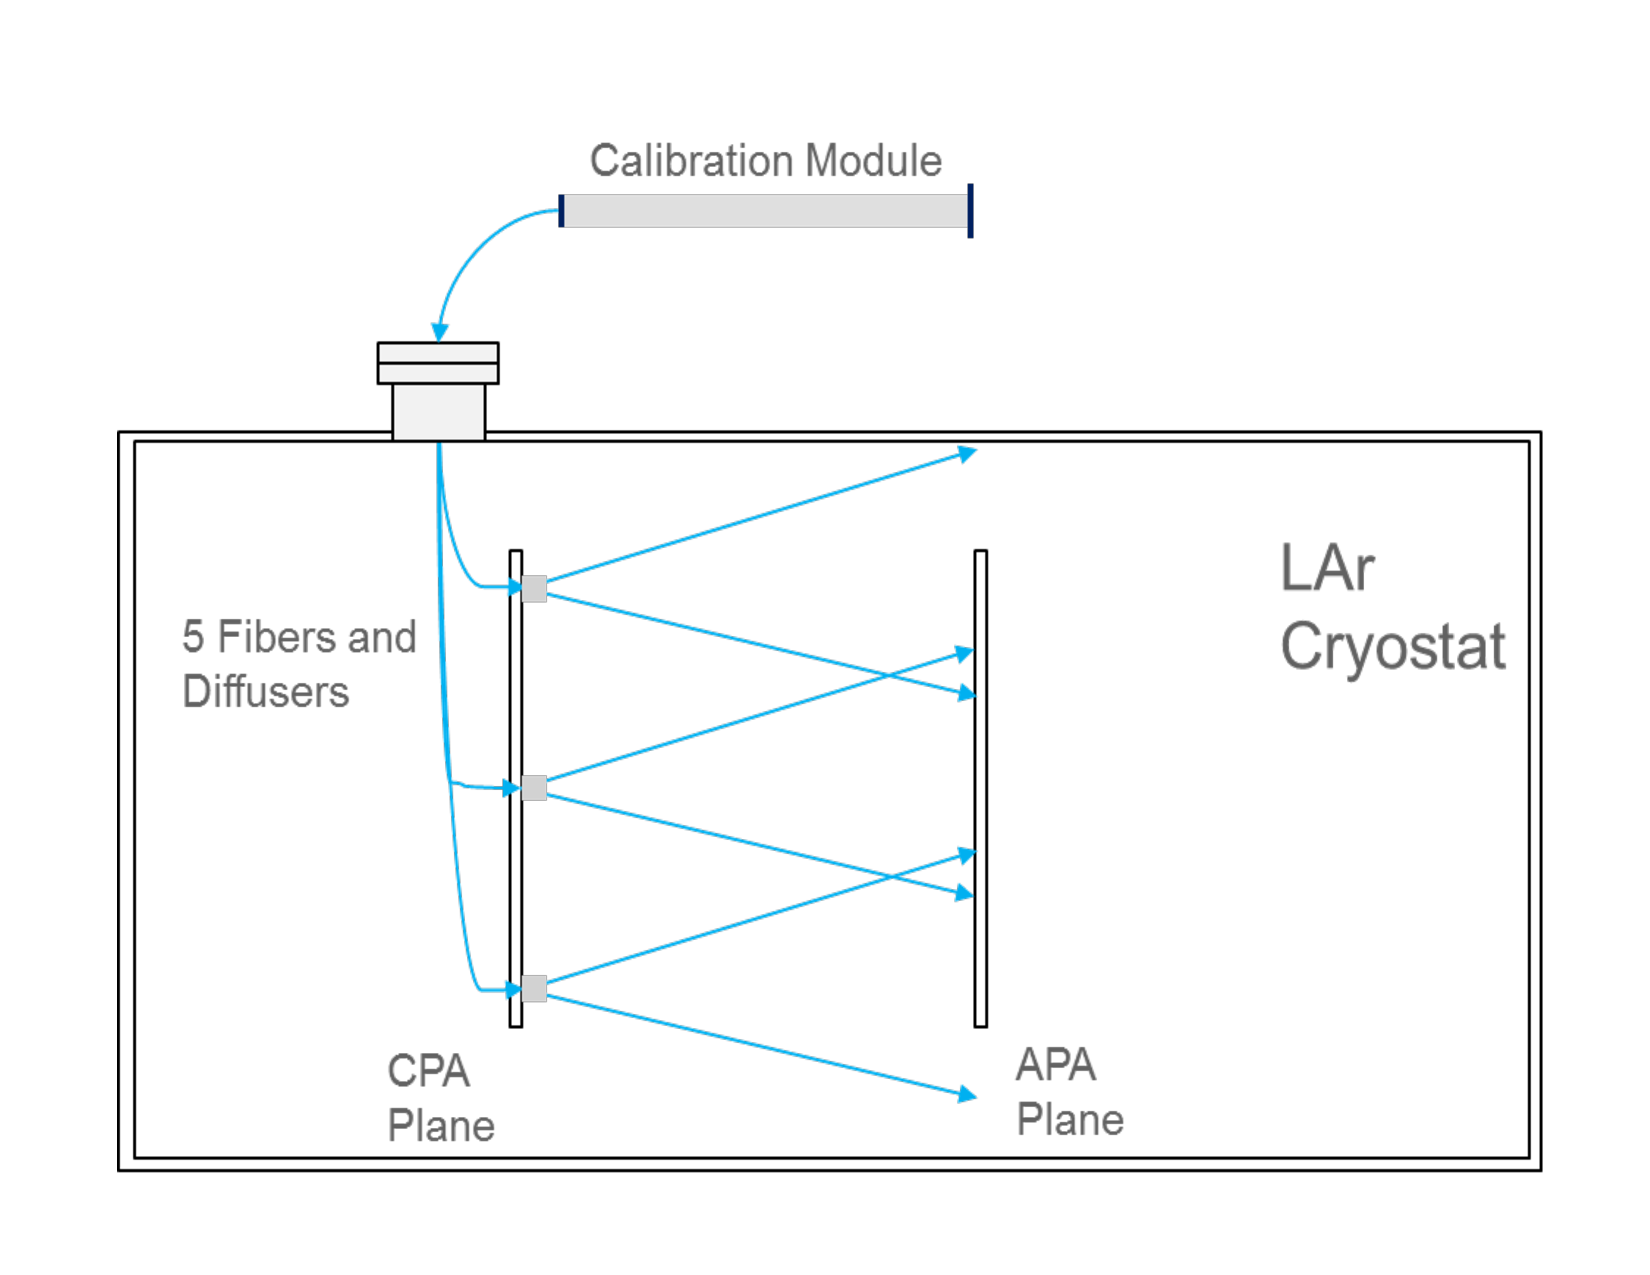
\includegraphics[angle=0,width=10cm,height=7cm]{calPD_concept-from-35ton.pdf}
\caption{Concept of the UV-light calibration system for the photon detector in liquid argon.}
\label{fig:fig-c-1}
\end{figure}
%
%
 \begin{figure}[h]
  \centering
%\includegraphics[angle=0,width=10cm,height=7cm]{fig-c-2.png}
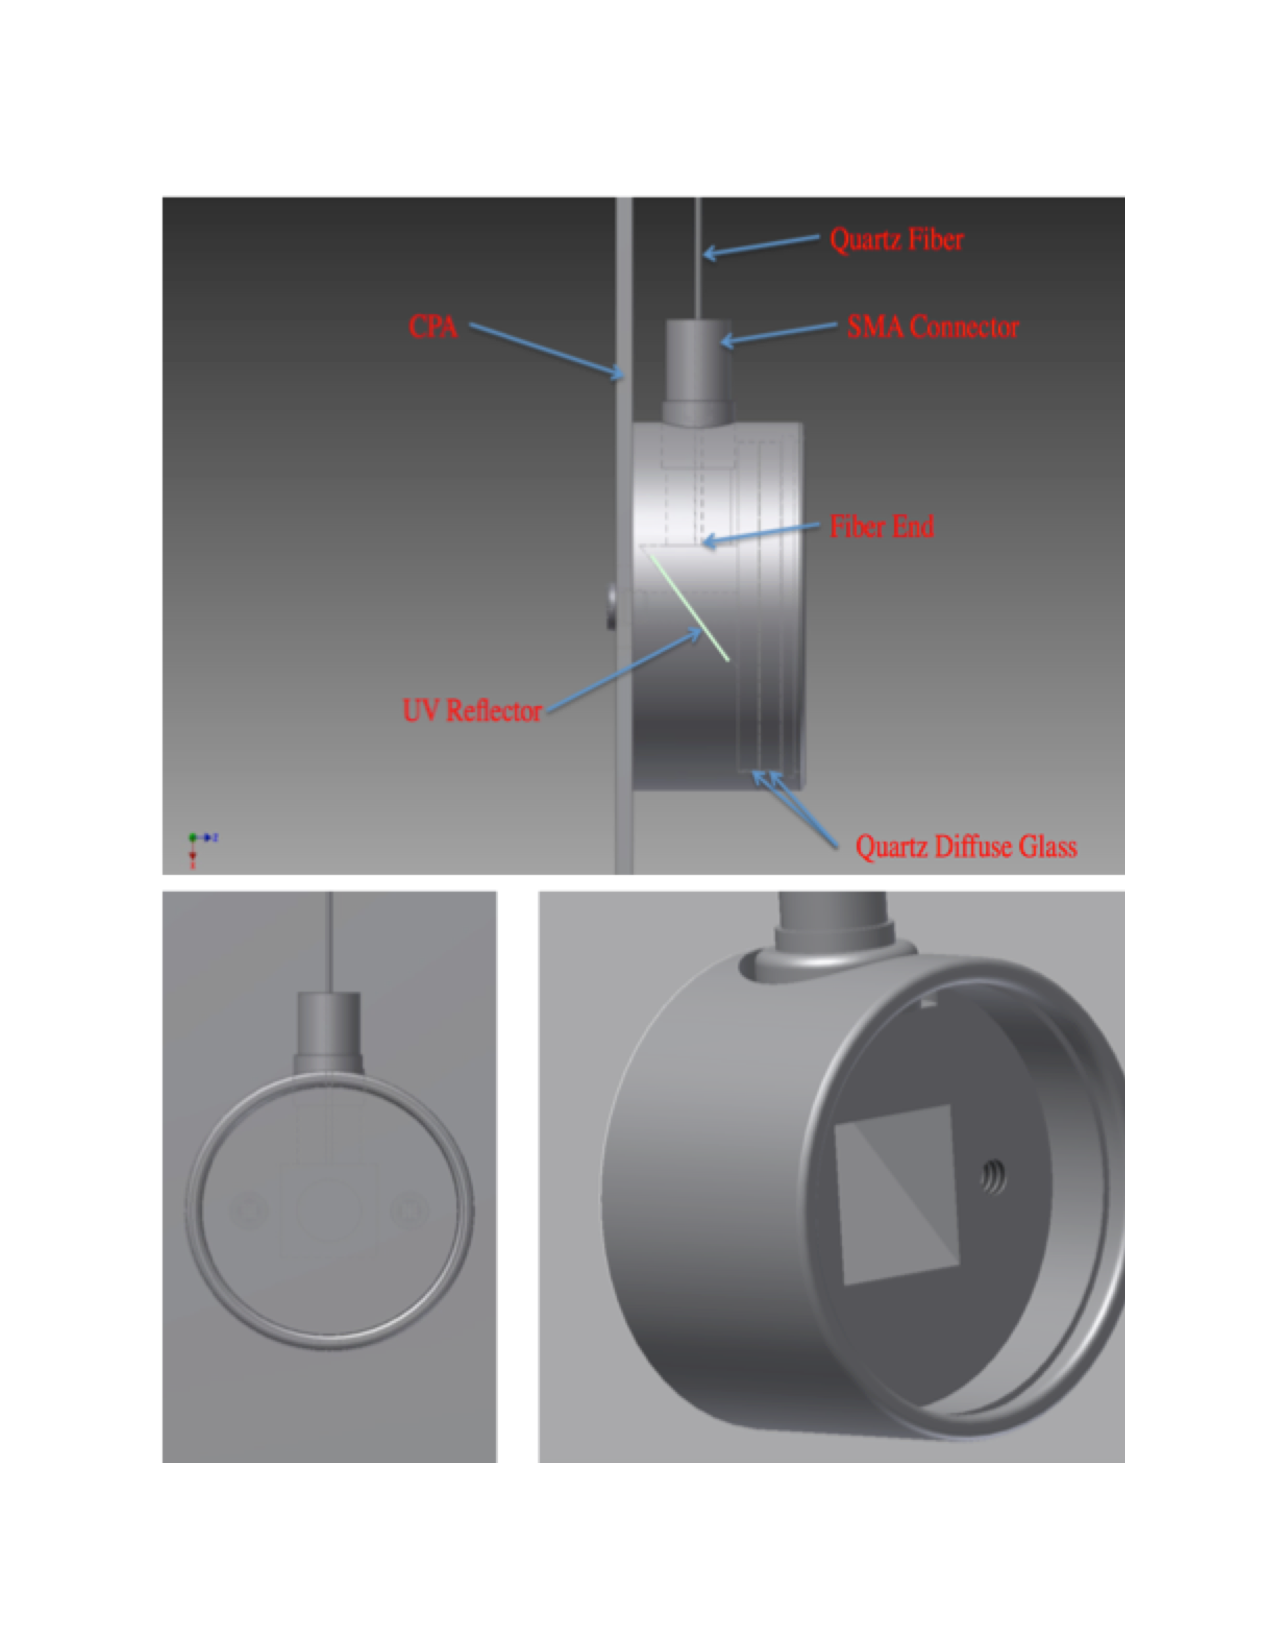
\includegraphics[angle=0,width=6cm,height=7cm]{calPD_Calibration_diffuser_system_protoDUNE_slide_left_half.pdf}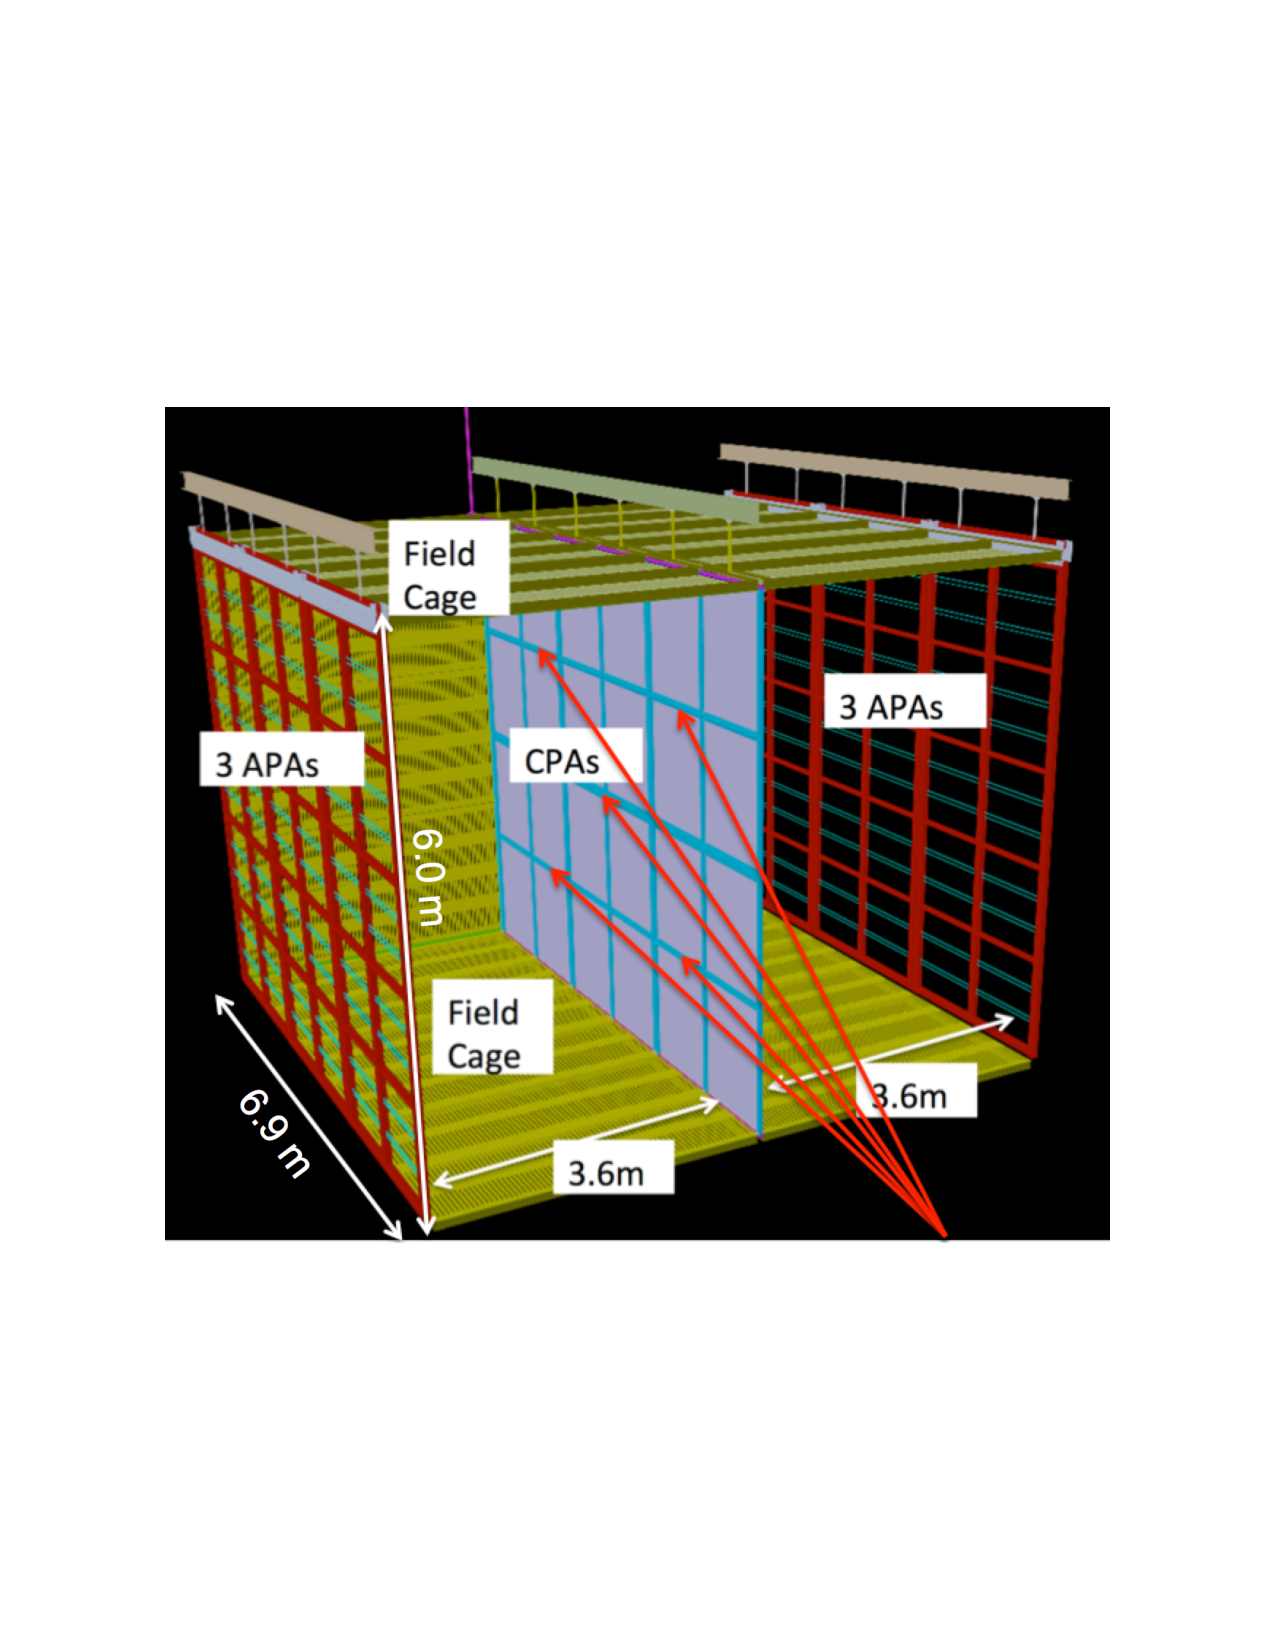
\includegraphics[angle=0,width=8cm,height=8cm]{calPD_Calib_diffuser_locations_protoDUNE.pdf}
\caption{The diffuse light is emitted from diffusers (top and bottom left figure) mounted at five CPA locations, indicated by arrows (right figure). 
The UV light from the light calibration system to diffusers is transported through quartz fiber.}
\label{fig:fig-c-2}
\end{figure}
%
%
For the 280 nm light we have performed a simulation of the designed diffuse light calibration system using TracePro, a generalized 3-D light ray-tracing program with the ability 
to include bulk optical properties such as absorption, fluorescence, birefringence in addition to surface properties such as scattering and reflection. 
As an example, in Fig.~\ref{fig:fig-c-4} we show simulated light distributions of at an APA surface for the cases of the VUV light emitted by either the central diffuser only (left figure), 
or by outer four diffusers simultaneously (right figure). 
%A full Geant4 based simulation of the detector will be used in the future. 
%Using the preliminary data with the 35-ton style light guides (indicating 0.5\% efficiency for number of photo-electrons per incident 128 nm LAr scintillation photon 50 cm from the light guide), we estimate for 280 nm light to observe ~15 photo-electrons per single SiPM channel when the light is emitted from the single central diffuser in 13 ns long pulses. Similarly, we expect about ~100 photo-electrons observed by a single SiPM channel when 280 nm light is emitted in 100 ns long pulses from the four outer diffusers at once.

%
 \begin{figure}[h]
  \centering
%\includegraphics[angle=0,width=6.5cm,height=3.5cm]{fig-c-4-L.png}\includegraphics[angle=0,width=6.5cm,height=3.5cm]{fig-c-4-R.png}
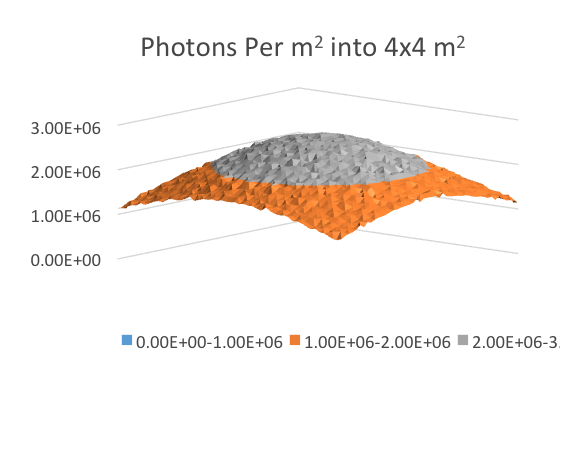
\includegraphics[angle=0,width=6.5cm,height=6cm]{calPD_4mx4m-area-3point6m-away-quantified.png}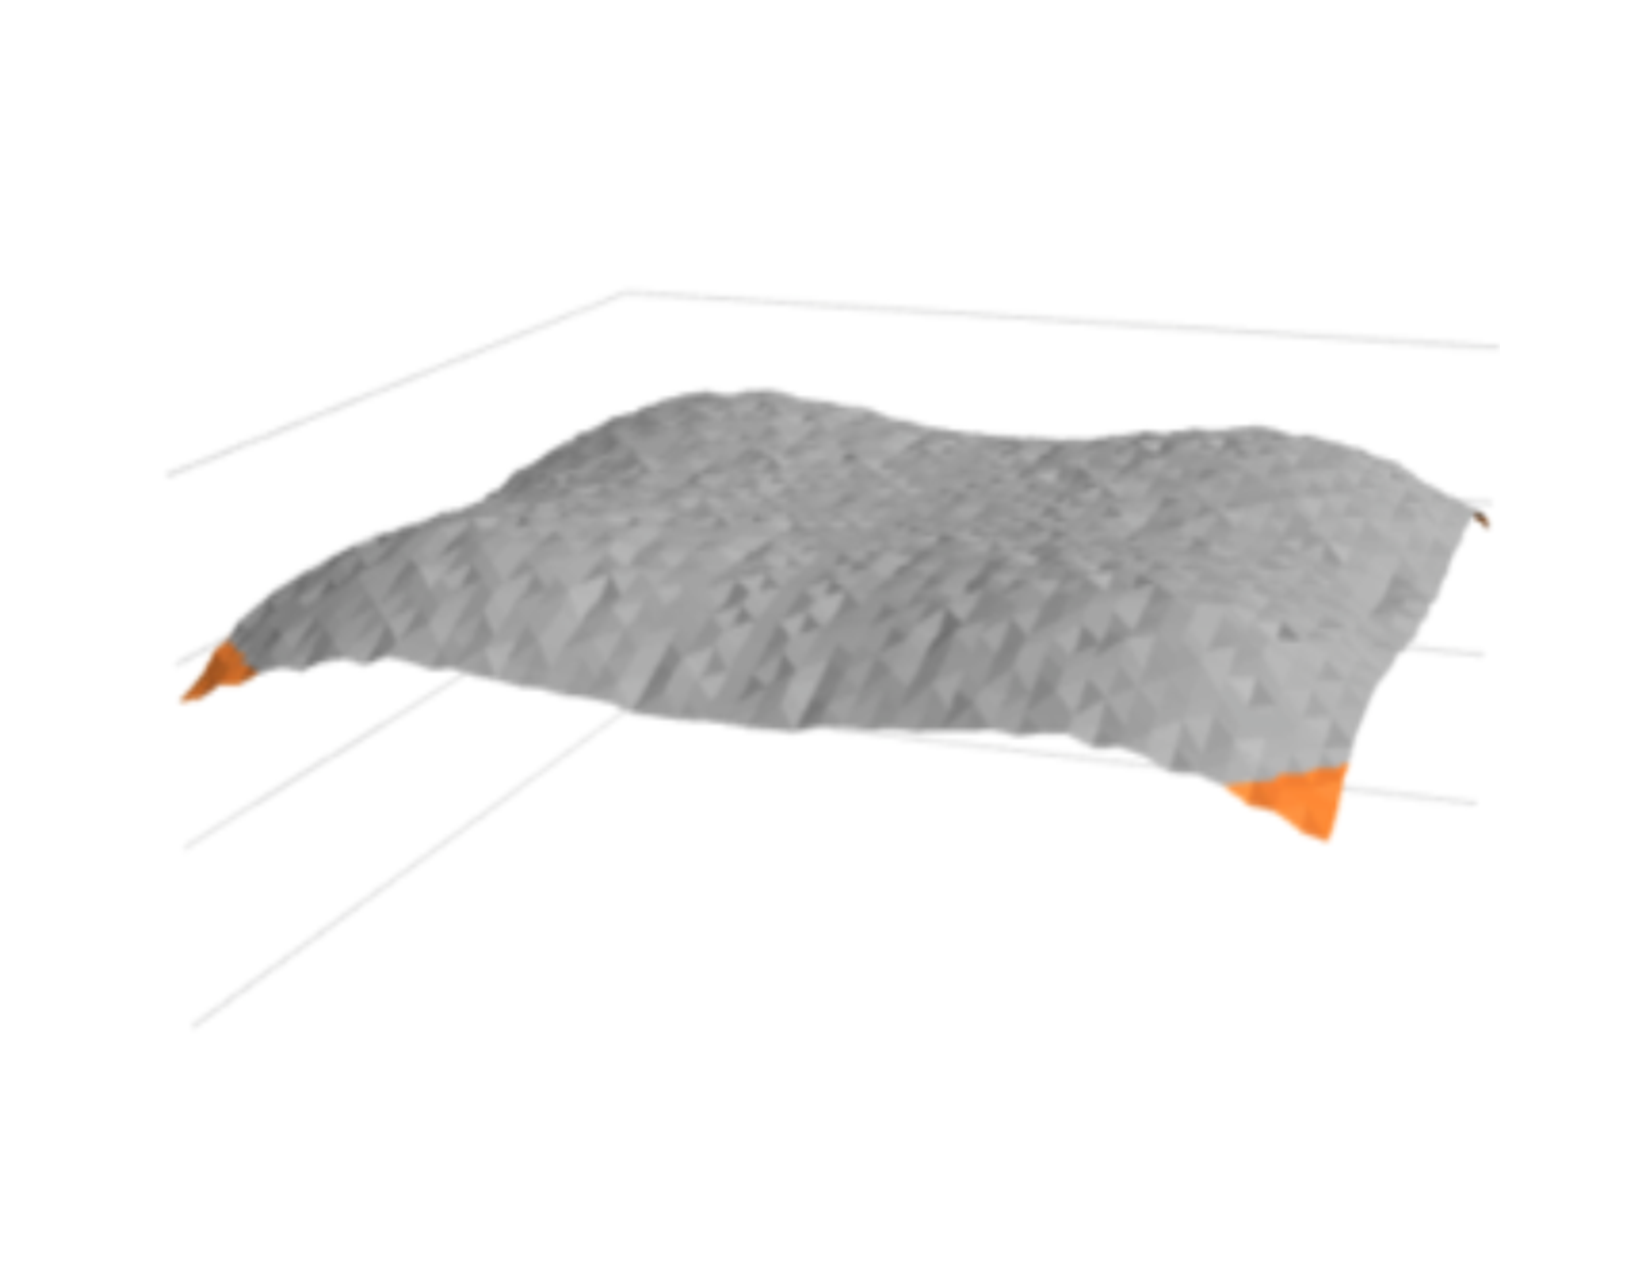
\includegraphics[angle=0,width=6.5cm,height=6cm]{calPD_figR.pdf}
\caption{Simulated light distributions of at the APA location for the cases of the VUV light emitted by either the central diffuser only (left figure), or by outer four diffusers simultaneously (right figure).
The simulation estimate has been obtained for 35-ton detector and scaled by to 3.6 m CPA - APA distance at protoDUNE.}
\label{fig:fig-c-4}
\end{figure}
%

The LCM module as well as the full prototype of the light calibration system system has been built, tested and successfully operated with 35-ton LAr TPC at Fermilab. The LCM is shown in Fig.~\ref{fig:fig-c-3}. 
The ANL photon calibration module combines the logic developed with the photon-detector readout electronics (so-called "SSP") unit.  An SSP board was essentially repackaged into a deeper rack mount 
chassis that accommodated a new internal LED Pulser Module (LPM) and an additional bulk power supply. The LPM utilizes five digital outputs to control the LPM pulse and its duration.  
These outputs are derived from the charge injection control logic within the SSP's FPGA.  The even channel SiPM bias DACs are used to control the LPM pulse amplitude.  
The adjacent odd channels are used to readout a reference photodiode which is used for pulse-by-pulse monitoring of the LED light output.  The output of the monitoring diode may be used to normalize 
the response of the SiPMs in the detector to the calibration pulse.

%
 \begin{figure}[h]
  \centering
%\includegraphics[angle=0,width=10cm,height=7cm]{fig-c-3.png}
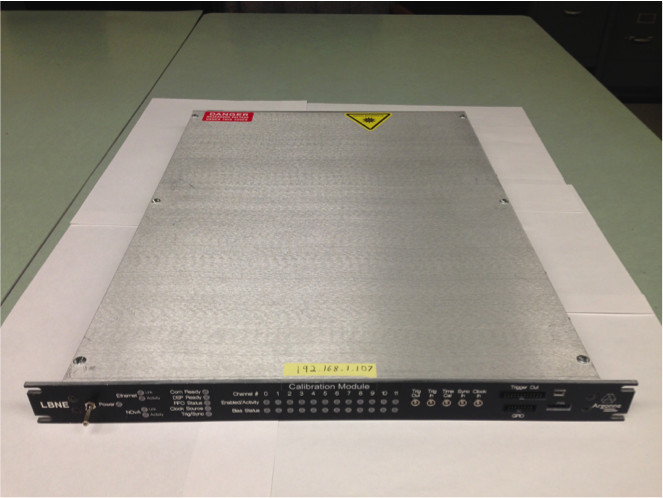
\includegraphics[angle=0,width=7cm,height=4.5cm]{calPD_LCM_front.png}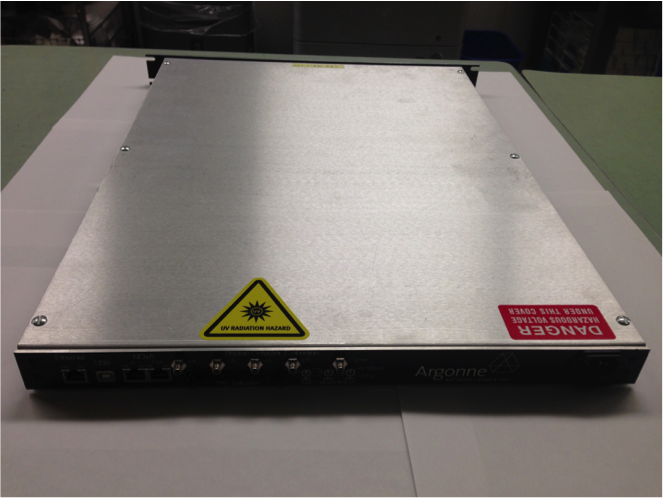
\includegraphics[angle=0,width=7cm,height=4.5cm]{calPD_LCM_back.png}
\caption{Photon detector light calibration module front (left figure) and back (right figure) ends.}
\label{fig:fig-c-3}
\end{figure}

%say it was realized already!!!
A prototype of the light calibration monitoring system described above has been designed, tested, installed, integrated, and operated with the 35-ton DUNE prototype detector.
The data is currently being analyzed. As en example of the system tests in former 35-ton detector in Fig.~\ref{fig:fig-wf} we show SSP waveforms collected as a response to the light calibration system described here.
This data has been collected in liquid argon, with the TPC powered-on, with the nominal value of drift high-voltage at 35-ton detector. The length of optical fiber cables used with the 35-ton detector 
was ~22 m total, including external fibers (7 m long), fiber feed-through, and internal fibers (15 m long).

%
 \begin{figure}[hhh!!!]
  \centering
%\includegraphics[angle=0,width=10cm,height=7cm]{fig-c-3.png}
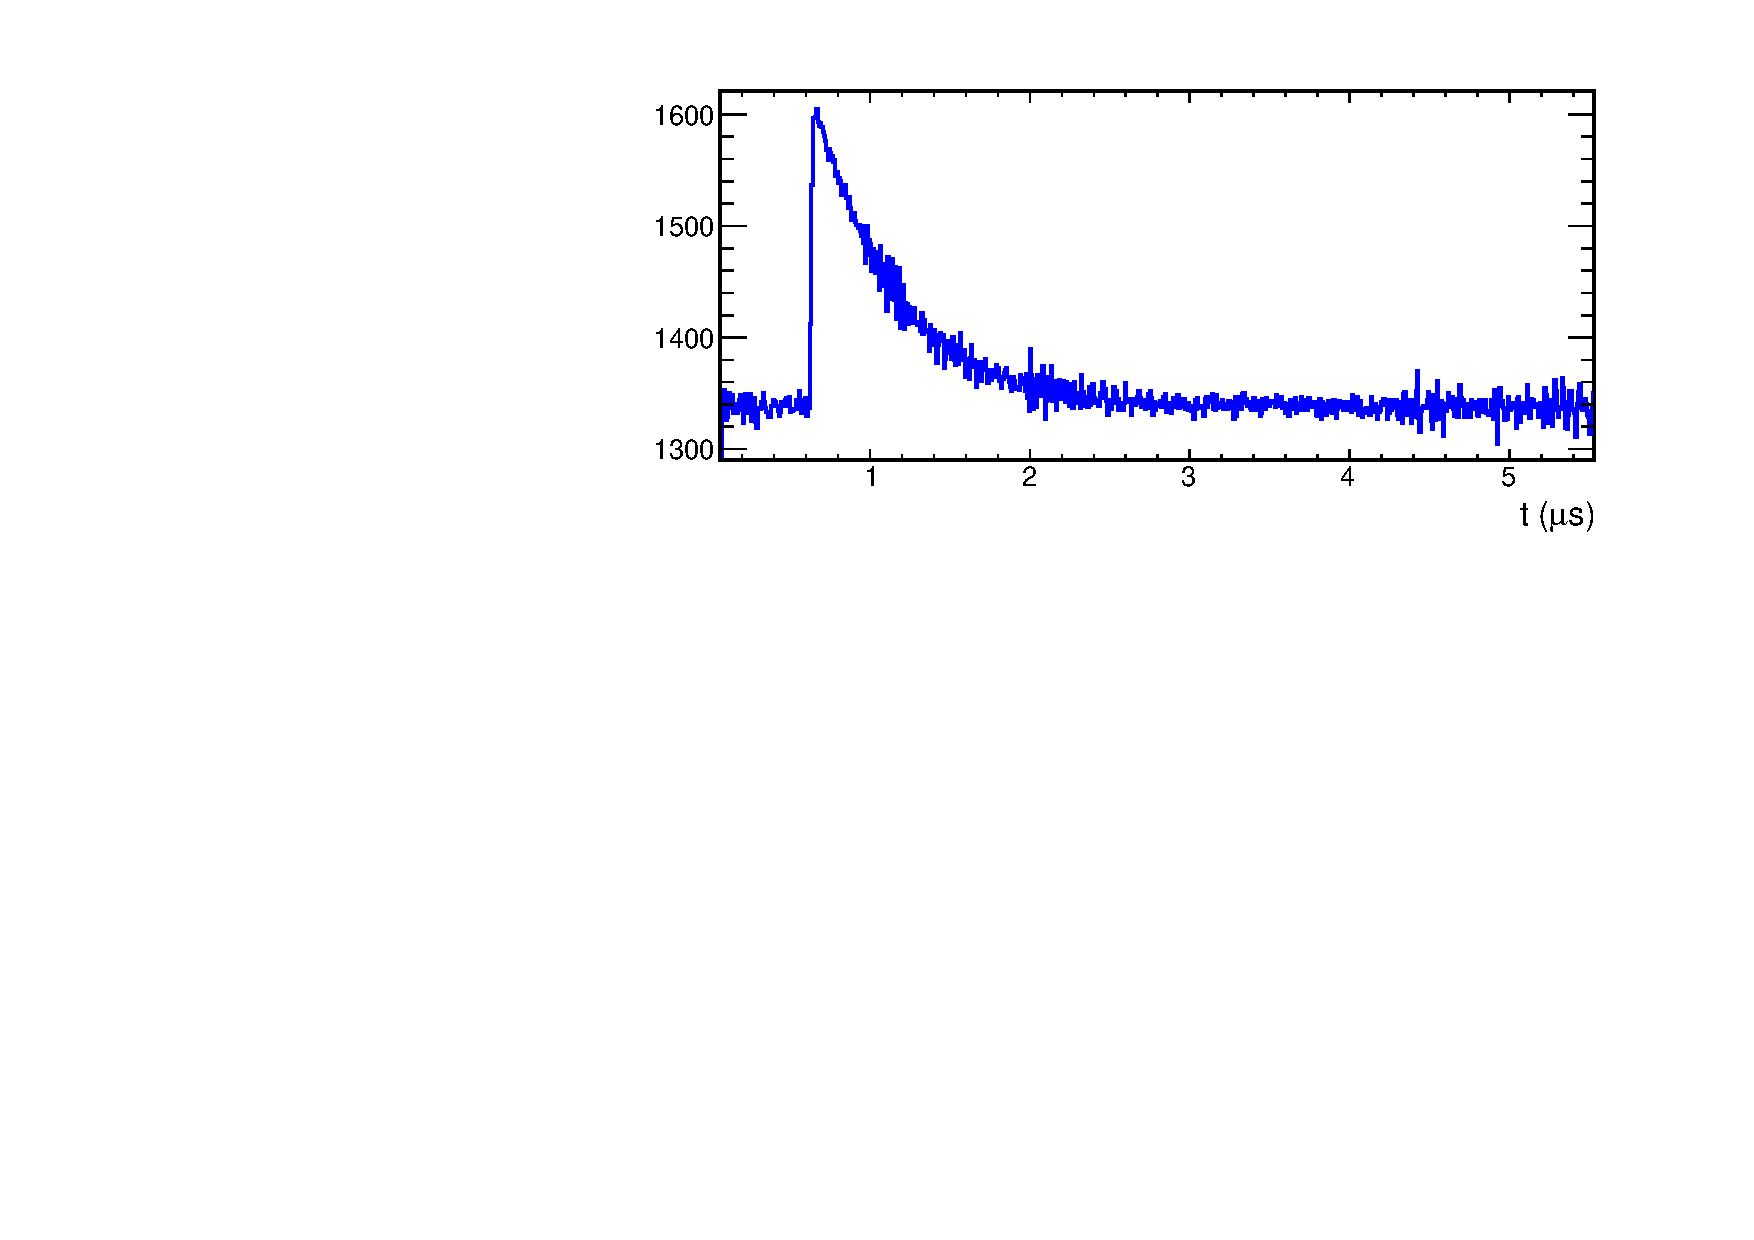
\includegraphics[angle=0,width=5cm,height=4cm]{calPD_example_ch21_run18573.pdf}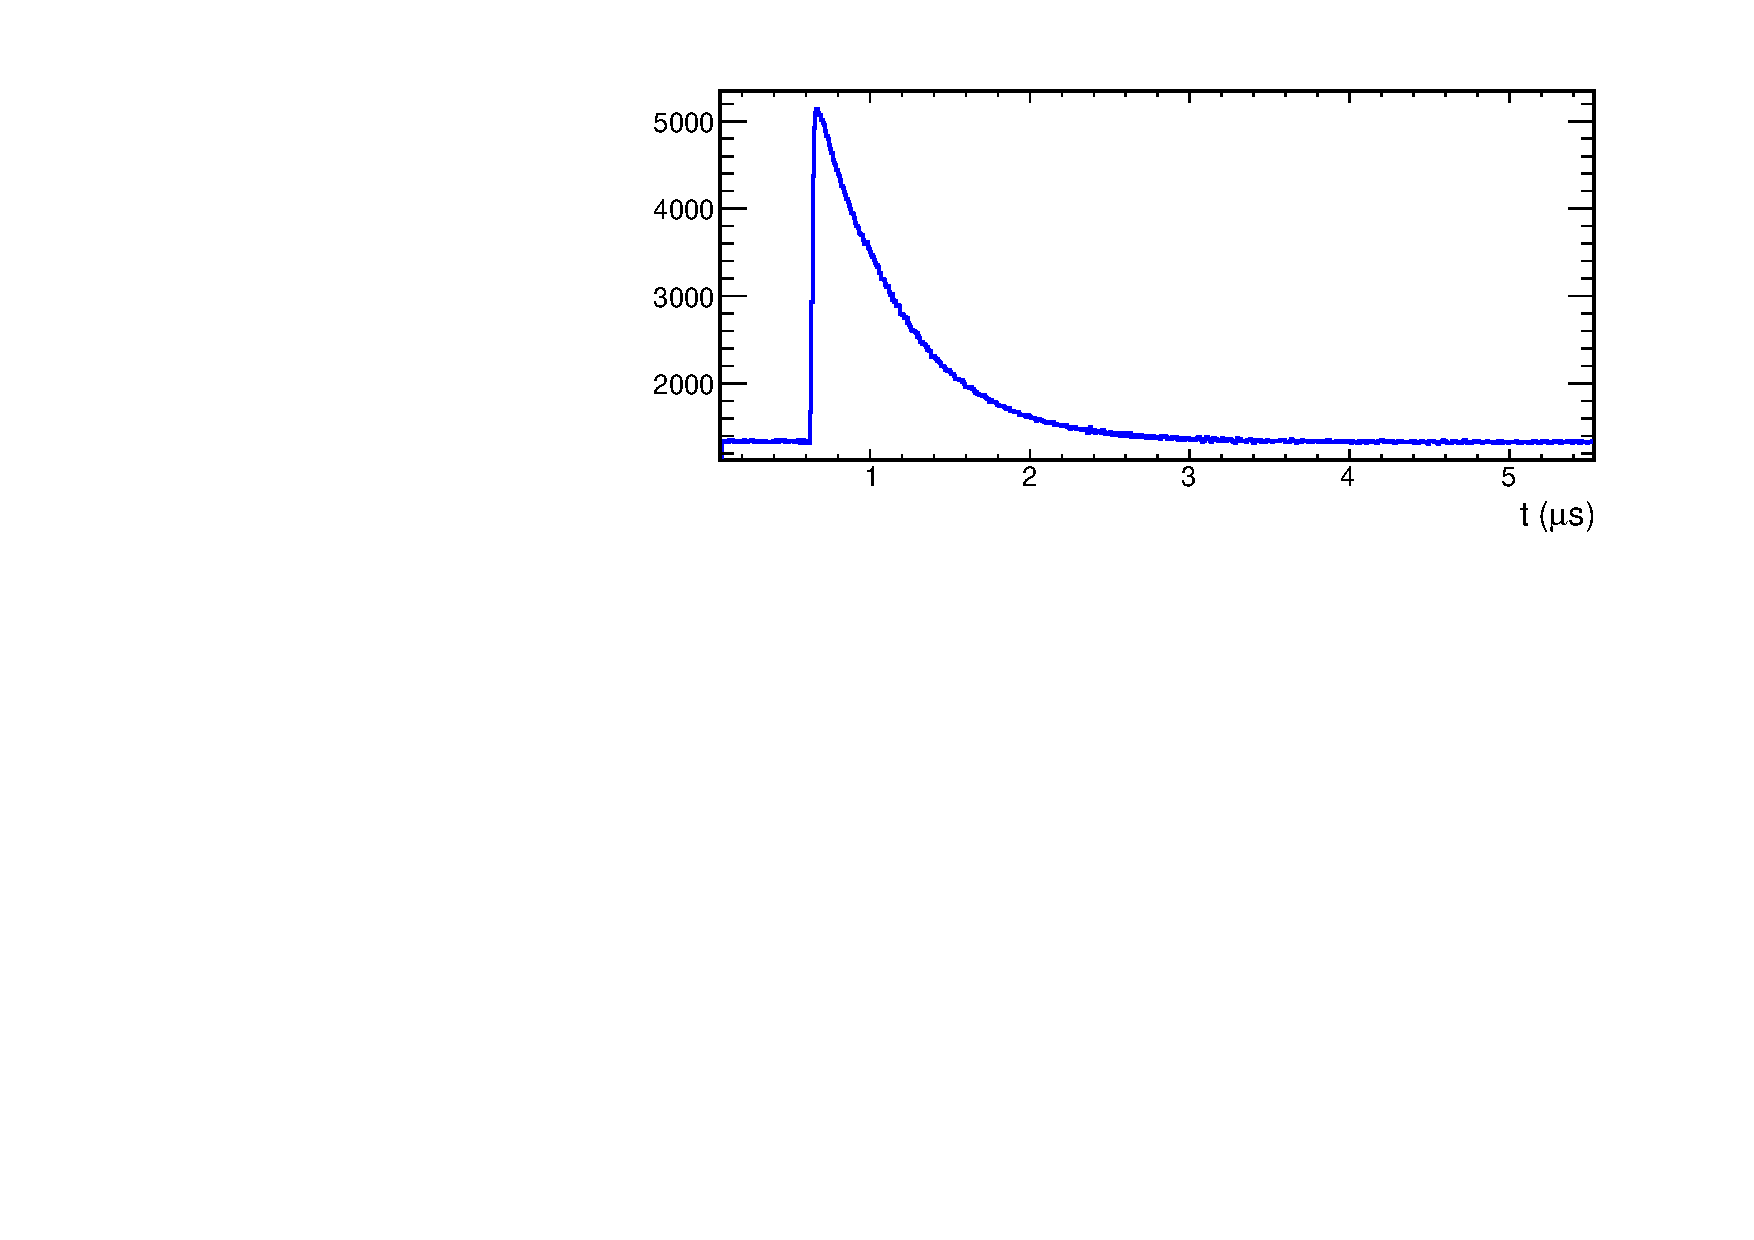
\includegraphics[angle=0,width=5cm,height=4cm]{calPD_example_ch21_run18574.pdf}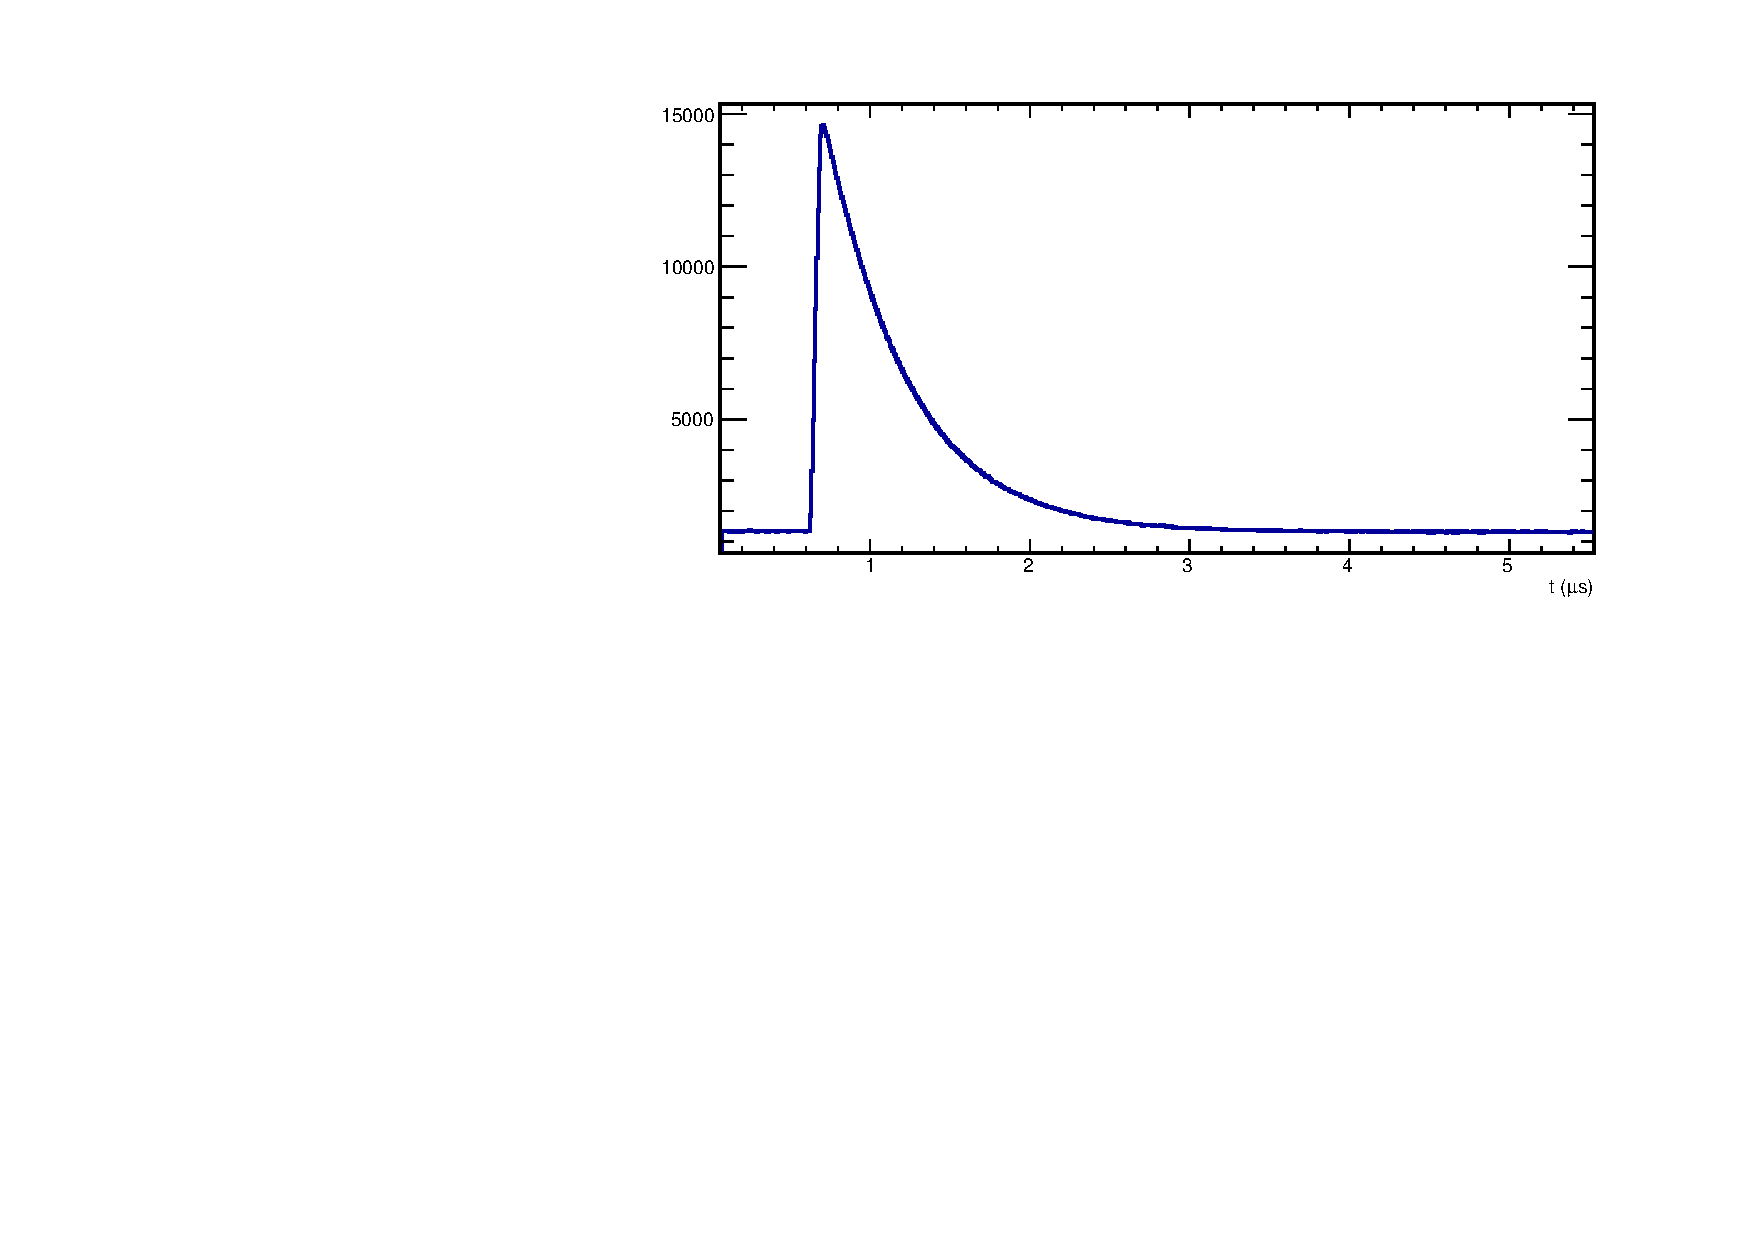
\includegraphics[angle=0,width=5cm,height=4cm]{calPD_example_ch21_run18572.pdf}
\caption{Photon detector light calibration pulses detected by readout electronics. Recorded waveforms have range from few photo-electrons (left figure), to tens of photo-electrons (middle figure), to hundreds of photo-electrons (right figure).}
\label{fig:fig-wf}
\end{figure}
%
In the DUNE prototypes (i.e. the protoDUNE) and in future DUNE Far Detectors it will be important to check if photon-detector components are functioning properly at various stages of the detector operation. 
Periodic light source deployments will monitor the systems stability as a function of time. A change in relative difference of UV light responses will point towards potential wave-length shifter instability, 
changes in SiPM gain and/or collection efficiencies. Much of the same monitoring is expected to be doable with cosmic rays in the protoDUNE (at surface), with periodic LED calibration runs complemented 
with cosmic-ray data tracked with an external hodoscope. With the protoDUNE detector one could use a well-defined muon trajectory defined by the hodoscope geometry and monitor the number 
of PEs per MeV of deposited charge. The number of PEs per photon-detector channel from the well-defined muon track could be used as a calibration constant. However, for the deep underground DUNE detectors the cosmic ray flux may inadequate for timely monitoring of the photon detectors.
	With the protoDUNE detector we have planned two sets of calibration runs: 
\begin{enumerate}
\item Calibration runs with four outer diffusers run simultaneously, in order to\\
-measure response of PD channels in multi-PE range and get integrated number of event samples for each channel (for maximum light output)\\
-test of the dynamic range from 1PE to maximum number of PEs. \\ 
-repeat runs periodically to trace any changes in channel response.
      
\item Runs with central diffuser only, in order to\\
-perform initial calibration runs that will reveal malfunctioning channels, if any.\\
-timing measurements with the 10-50 ns pulses, verify time resolution of the PD system.
\end{enumerate}

The controlled source of light described here will be used to perform a relative "t0" calibration, where the "t0" could be absolutely calibrated with the use of the cosmic 
ray triggers available with protoDUNE detector. Effects that contribute to a finite time resolution and relative time offset of photon-detector channels include scintillation time constants, 
photon conversion with wave-length shifter, photon propagation through photon-detector paddle, SiPM jitter, and FEE resolution. Most these effects are constant and can be individually 
measured on the bench, so the LED flasher system will monitor overall stability of the photon detector.
%	To go beyond the current R\&D phase one needs detailed MC simulations of light production, propagation, and detection to perform comparisons of reconstruction performance 
%against prototype data in terms of calorimetric energy and position reconstructions for measured event tracks. Future light collection systems will aim to maximize the active area of 
%the light guide bars, to achieve a high photon detection efficiency with an optimized timing and granularity required for improved position resolution. As in the case with the TPC charge 
%calibration we will need to evaluate what may be achieved with expected cosmic ray muons and Michel electrons, $\pi^0$, and natural radioactivity events 
%(such as $^{39}$Ar with end-point energy of abut 500 keV).


%\end{document}
